% ============================================================================
% Reporte de avance - Entrega 2 (Semana 5)
%
% Estructura tomada de la seccion "Entregables" de la guia del microproyecto.
% El reporte no puede superar 10 paginas (solo se califican las primeras 10).
% La seccion 1 tiene su propio limite de 1 pagina.
%
% Estado: contenido consolidado para el cierre de la Entrega 2.
% ============================================================================
\documentclass[11pt]{article}

% ======================= PAQUETES =======================
\usepackage[utf8]{inputenc}
\usepackage[T1]{fontenc}
\usepackage[spanish,es-tabla]{babel}
\usepackage{geometry}
\geometry{a4paper, top=2.8cm, bottom=2.8cm, left=2.6cm, right=2.6cm}

\usepackage{titlesec}
\usepackage{fancyhdr}
\usepackage{booktabs}
\usepackage{array}
\usepackage{enumitem}
\usepackage{xcolor}
\usepackage{tcolorbox}
\usepackage{graphicx}
\usepackage{hyperref}
\usepackage{parskip}
\usepackage{caption}

% ======================= COLORES =======================
\definecolor{primaryblue}{RGB}{28,58,92}
\definecolor{accentblue}{RGB}{47,109,161}
\definecolor{lightgray}{RGB}{245,246,248}
\definecolor{midgray}{RGB}{110,110,110}

% ======================= TÍTULOS DE SECCIÓN =======================
\titleformat{\section}
  {\Large\bfseries\color{primaryblue}}
  {\thesection.}{0.4em}{}
\titlespacing*{\section}{0pt}{1.4em}{0.6em}

\titleformat{\subsection}
  {\large\bfseries\color{accentblue}}
  {\thesubsection}{0.4em}{}
\titlespacing*{\subsection}{0pt}{1.0em}{0.4em}

% ======================= ENCABEZADO / PIE =======================
\pagestyle{fancy}
\fancyhf{}
\renewcommand{\headrulewidth}{0.4pt}
\renewcommand{\footrulewidth}{0pt}
\fancyhead[L]{\small\color{midgray} Recomendación local de citas académicas}
\fancyhead[R]{\small\color{midgray} Semana 5 -- Reporte de avance}
\fancyfoot[C]{\small\color{midgray} \thepage}

% ======================= HYPERREF =======================
\hypersetup{
  colorlinks=true,
  linkcolor=accentblue,
  citecolor=accentblue,
  urlcolor=accentblue,
  pdftitle={Recomendación local de citas académicas - Entrega 2},
  pdfauthor={Maestría en Inteligencia Artificial - Universidad de los Andes}
}

\newcommand{\notabox}[1]{%
  \begin{tcolorbox}[colback=lightgray, colframe=accentblue, boxrule=0.6pt,
    left=8pt, right=8pt, top=5pt, bottom=5pt, arc=2pt]
    \small #1
  \end{tcolorbox}
}

\begin{document}

% ======================= PORTADA =======================
\begin{titlepage}
\centering
\vspace*{2.5cm}

{\Large \color{midgray} Maestría en Inteligencia Artificial}\\[0.2cm]
{\large \color{midgray} Universidad de los Andes}\\[2.5cm]

{\color{primaryblue}\rule{\linewidth}{1.2pt}}\\[0.6cm]
{\Huge \bfseries \color{primaryblue} Recomendación local de citas\\ académicas mediante aprendizaje\\ automático}\\[0.6cm]
{\color{primaryblue}\rule{\linewidth}{1.2pt}}\\[0.8cm]

{\Large Reporte de avance del microproyecto -- Semana 5}\\[3cm]

\begin{tabular}{rl}
\textbf{Nombres participantes:} & Carlos Duque, Carlos Caicedo, Jose Zambrana, John Arias \\[4pt]
\textbf{Proyecto:} & Desarrollo de Soluciones \\[4pt]
\textbf{Docente:} & Juan Fernando Pérez \\[4pt]
\textbf{Fecha:} & 6 de septiembre de 2026 \\
\end{tabular}

\vfill
{\small \color{midgray} Universidad de los Andes -- Maestría en Inteligencia Artificial}
\end{titlepage}

% ============================================================================
% 1. RESUMEN DEL PROBLEMA
% ============================================================================
\section{Resumen del problema}

\subsection{Contexto}

El crecimiento sostenido de la literatura científica dificulta que investigadores y autores identifiquen con rapidez los trabajos pertinentes para respaldar una afirmación mientras redactan. La recomendación local de citas aborda el problema usando como consulta el contexto textual próximo al lugar donde se requiere la referencia, y ordenando artículos candidatos por su relevancia frente a ese fragmento (Gu, Gao y Hahnloser, 2022).

\subsection{Pregunta de negocio y alcance}

\notabox{¿Cómo apoyar a un autor de textos académicos en la identificación de artículos potencialmente relevantes para citar, utilizando el contexto textual local en el que requiere incluir una referencia?}

El alcance del microproyecto es un prototipo funcional que recibe un contexto académico en inglés y devuelve un ranking de artículos candidatos con su puntaje de relevancia, servido por una API y consumido por un tablero interactivo.

\subsection{Conjuntos de datos}

Se emplea el conjunto \texttt{custom} (ACL-200) del repositorio \textit{Local-Citation-Recommendation}: 63.768 contextos de cita, 19.776 artículos con título y resumen, y particiones de entrenamiento, validación y prueba con 30.390, 9.381 y 9.585 consultas respectivamente. Los datos se versionan con DVC sobre almacenamiento S3.

\subsection{Cambios respecto a la primera entrega}

\begin{itemize}[leftmargin=1.4em, itemsep=1pt, topsep=2pt]
  \item \textbf{Arquitectura de recuperación en dos etapas.} La Entrega 1 planteaba un único modelo supervisado que estimara la relevancia de cada candidato. La medición de la línea base mostró que puntuar los 19.776 artículos por consulta es inviable en tiempo interactivo, por lo que el diseño pasó a una primera etapa de recuperación léxica que reduce a los mejores candidatos y una segunda de reordenamiento supervisado sobre ese subconjunto.
  \item \textbf{Métricas de evaluación.} Se adoptaron Recall@K y MRR@K, propias de recuperación de información, en lugar de métricas de clasificación. Ambas se calculan truncadas a K, como es convención en el área.
  \item \textbf{Infraestructura de experimentación.} Se incorporó MLflow sobre una instancia EC2 para registrar y comparar todas las corridas de forma centralizada.
\end{itemize}

% ============================================================================
% 2. MODELOS DESARROLLADOS Y SU EVALUACION
% ============================================================================
\section{Modelos desarrollados y su evaluación}

\subsection{Protocolo de evaluación}

Todos los modelos se evalúan sobre las mismas 9.381 consultas de validación, contra el total de 19.776 artículos candidatos. Se reportan dos métricas, ambas truncadas a $K$:

\begin{itemize}[leftmargin=1.4em, itemsep=1pt, topsep=2pt]
  \item \textbf{Recall@K}: proporción de consultas cuyo artículo citado aparece entre las $K$ primeras posiciones. Mide si el sistema \textit{encuentra} el artículo correcto.
  \item \textbf{MRR@K}: inverso promedio de la posición del primer acierto. Mide si lo ubica \textit{arriba} en el ranking.
\end{itemize}

La distinción entre ambas resulta central para las conclusiones de la Sección 3.

\subsection{Línea base: TF-IDF con similitud coseno}

La línea base representa cada artículo (título más resumen) y cada contexto de cita como vectores TF-IDF, y ordena los artículos por similitud coseno con el contexto. No aprende de los ejemplos etiquetados: solo mide coincidencia léxica. Su función es fijar el piso de comparación que cualquier modelo supervisado debe superar para justificarse.

Sobre la configuración de referencia (vocabulario de 25.305 términos, \texttt{min\_df} igual a 2) los resultados son:

\begin{table}[h!]
\centering
\small
\caption{Desempeño de la línea base TF--IDF según la profundidad del ranking}
\label{tab:curva}
\begin{tabular}{c c c}
\toprule
\textbf{K} & \textbf{Recall@K} & \textbf{MRR@K} \\
\midrule
1   & 0,0770 & 0,0770 \\
5   & 0,1887 & 0,1161 \\
10  & 0,2541 & 0,1249 \\
20  & 0,3238 & 0,1298 \\
50  & 0,4282 & 0,1330 \\
100 & 0,5163 & 0,1343 \\
\bottomrule
\end{tabular}
\end{table}

\begin{figure}[h!]
\centering
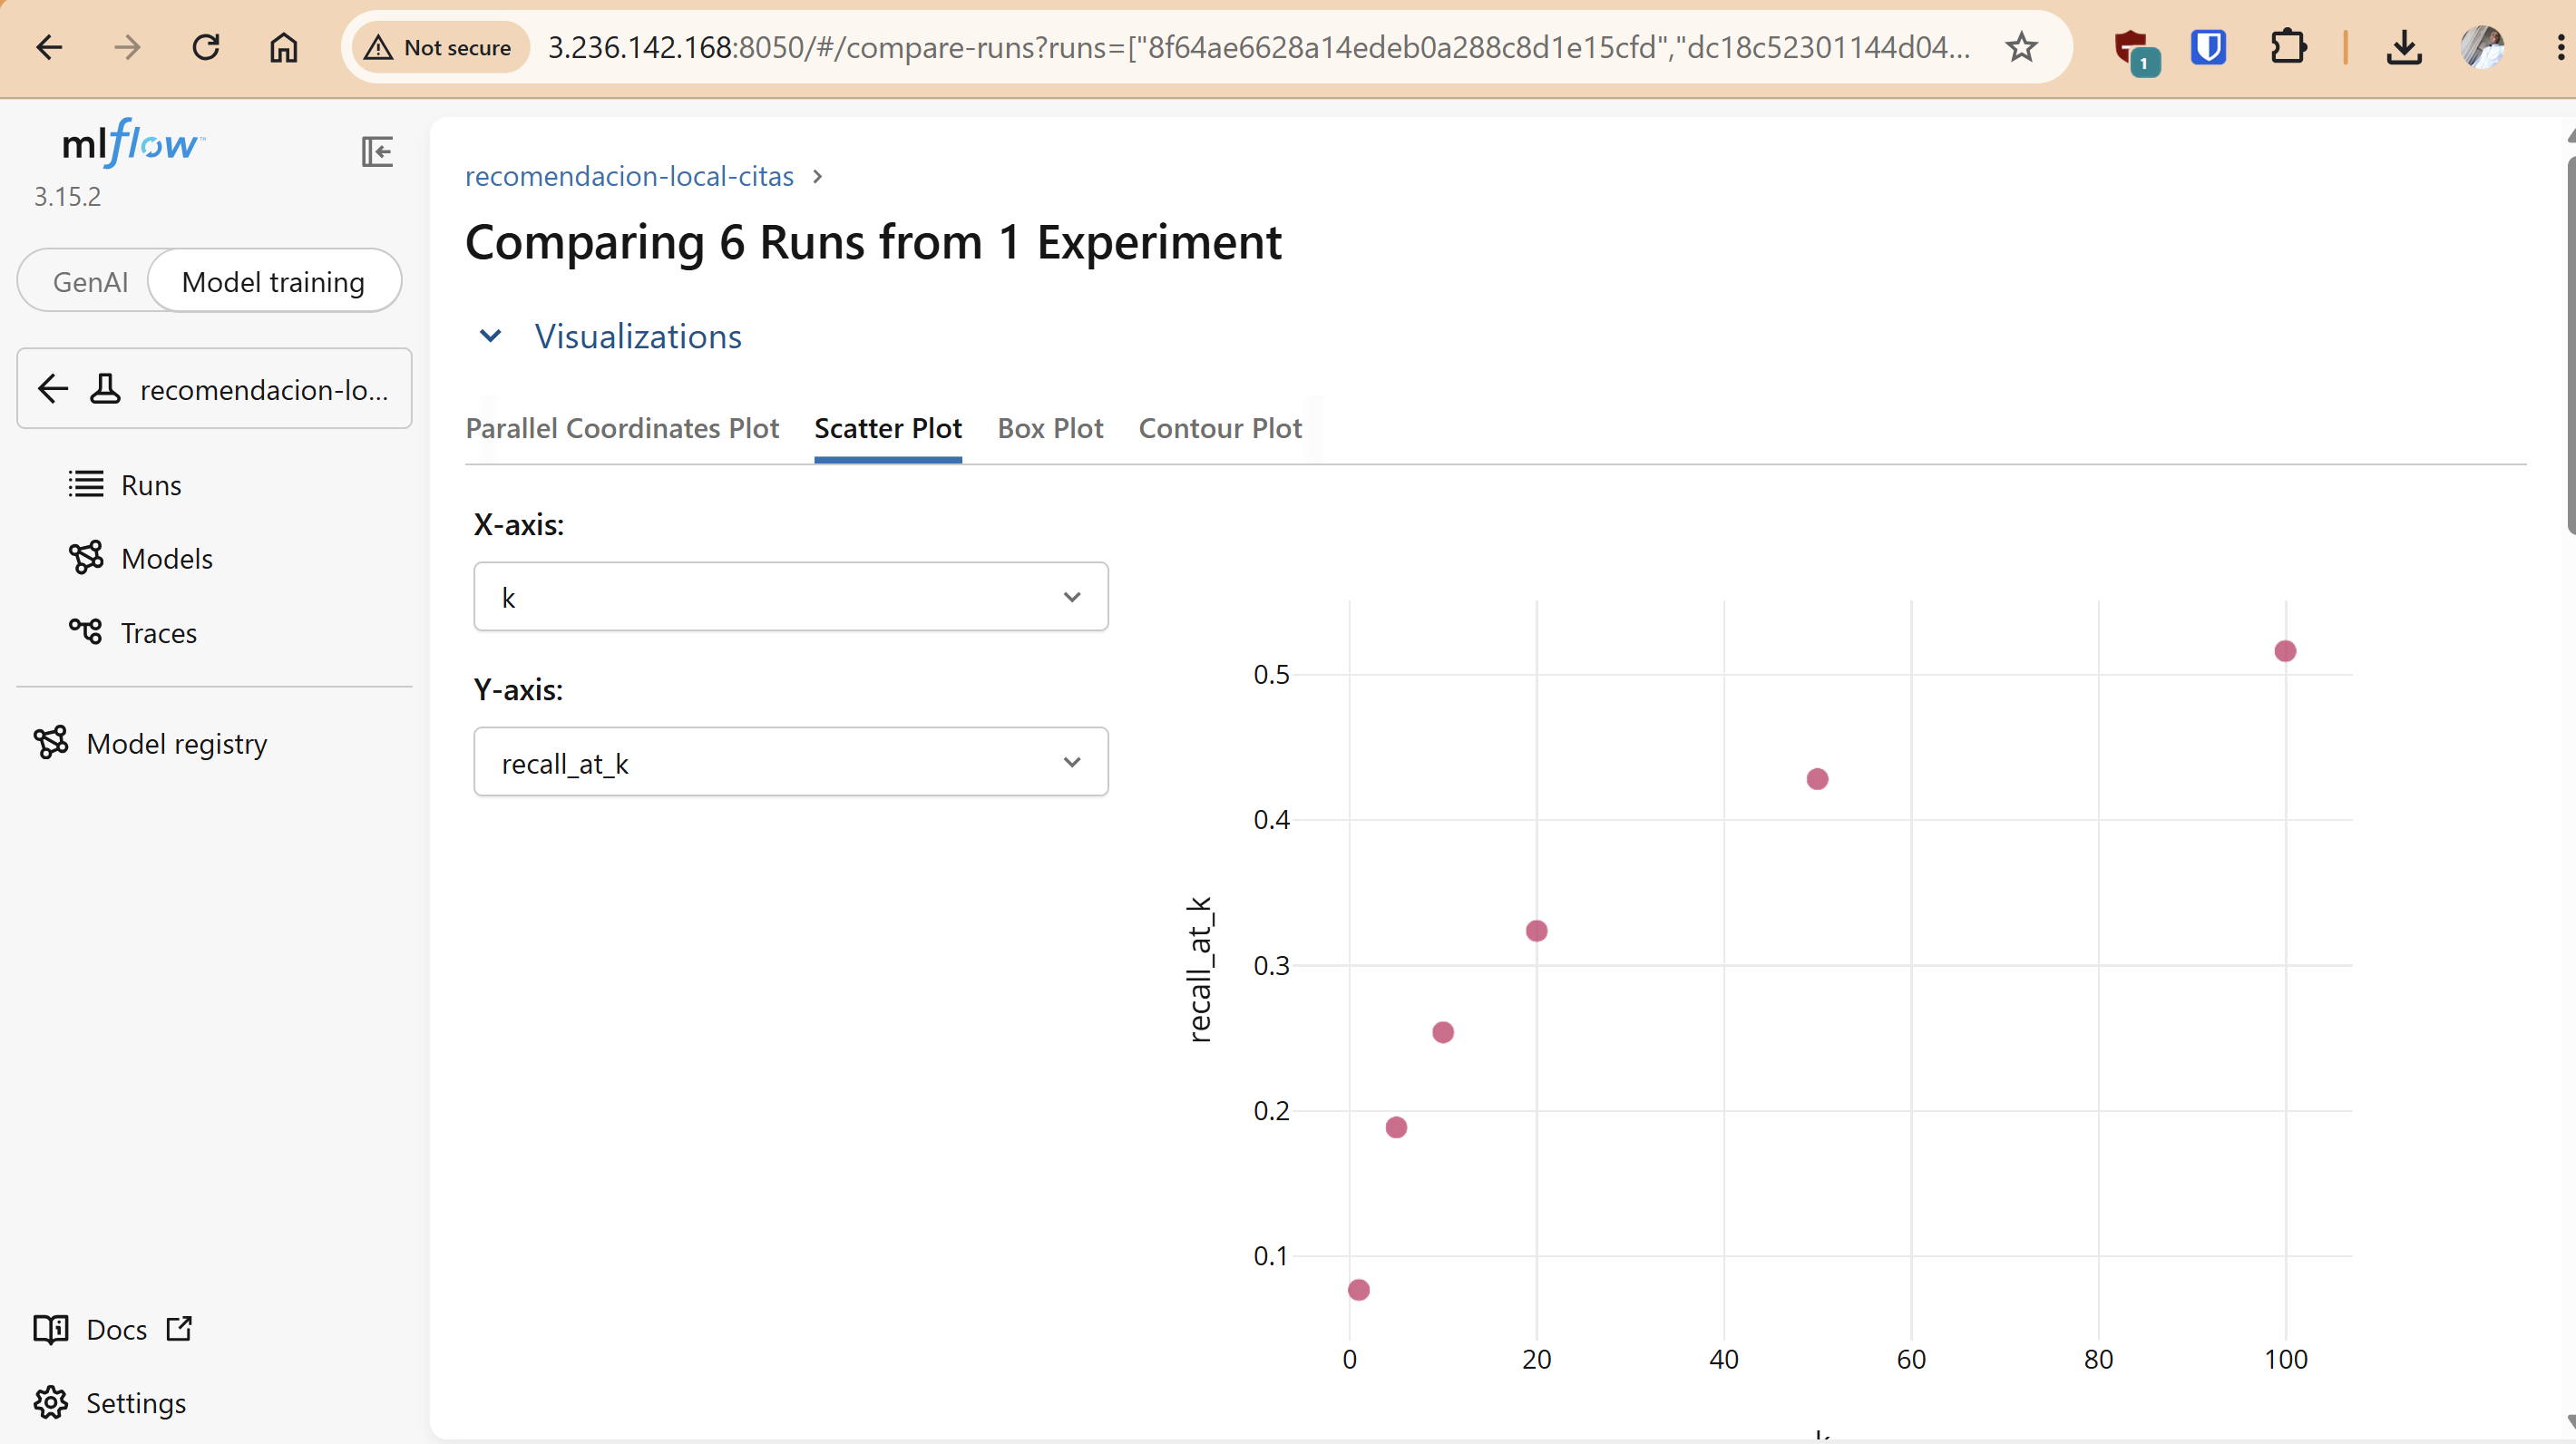
\includegraphics[width=0.48\textwidth]{mlflow_curva_recall_k.png}
\hfill
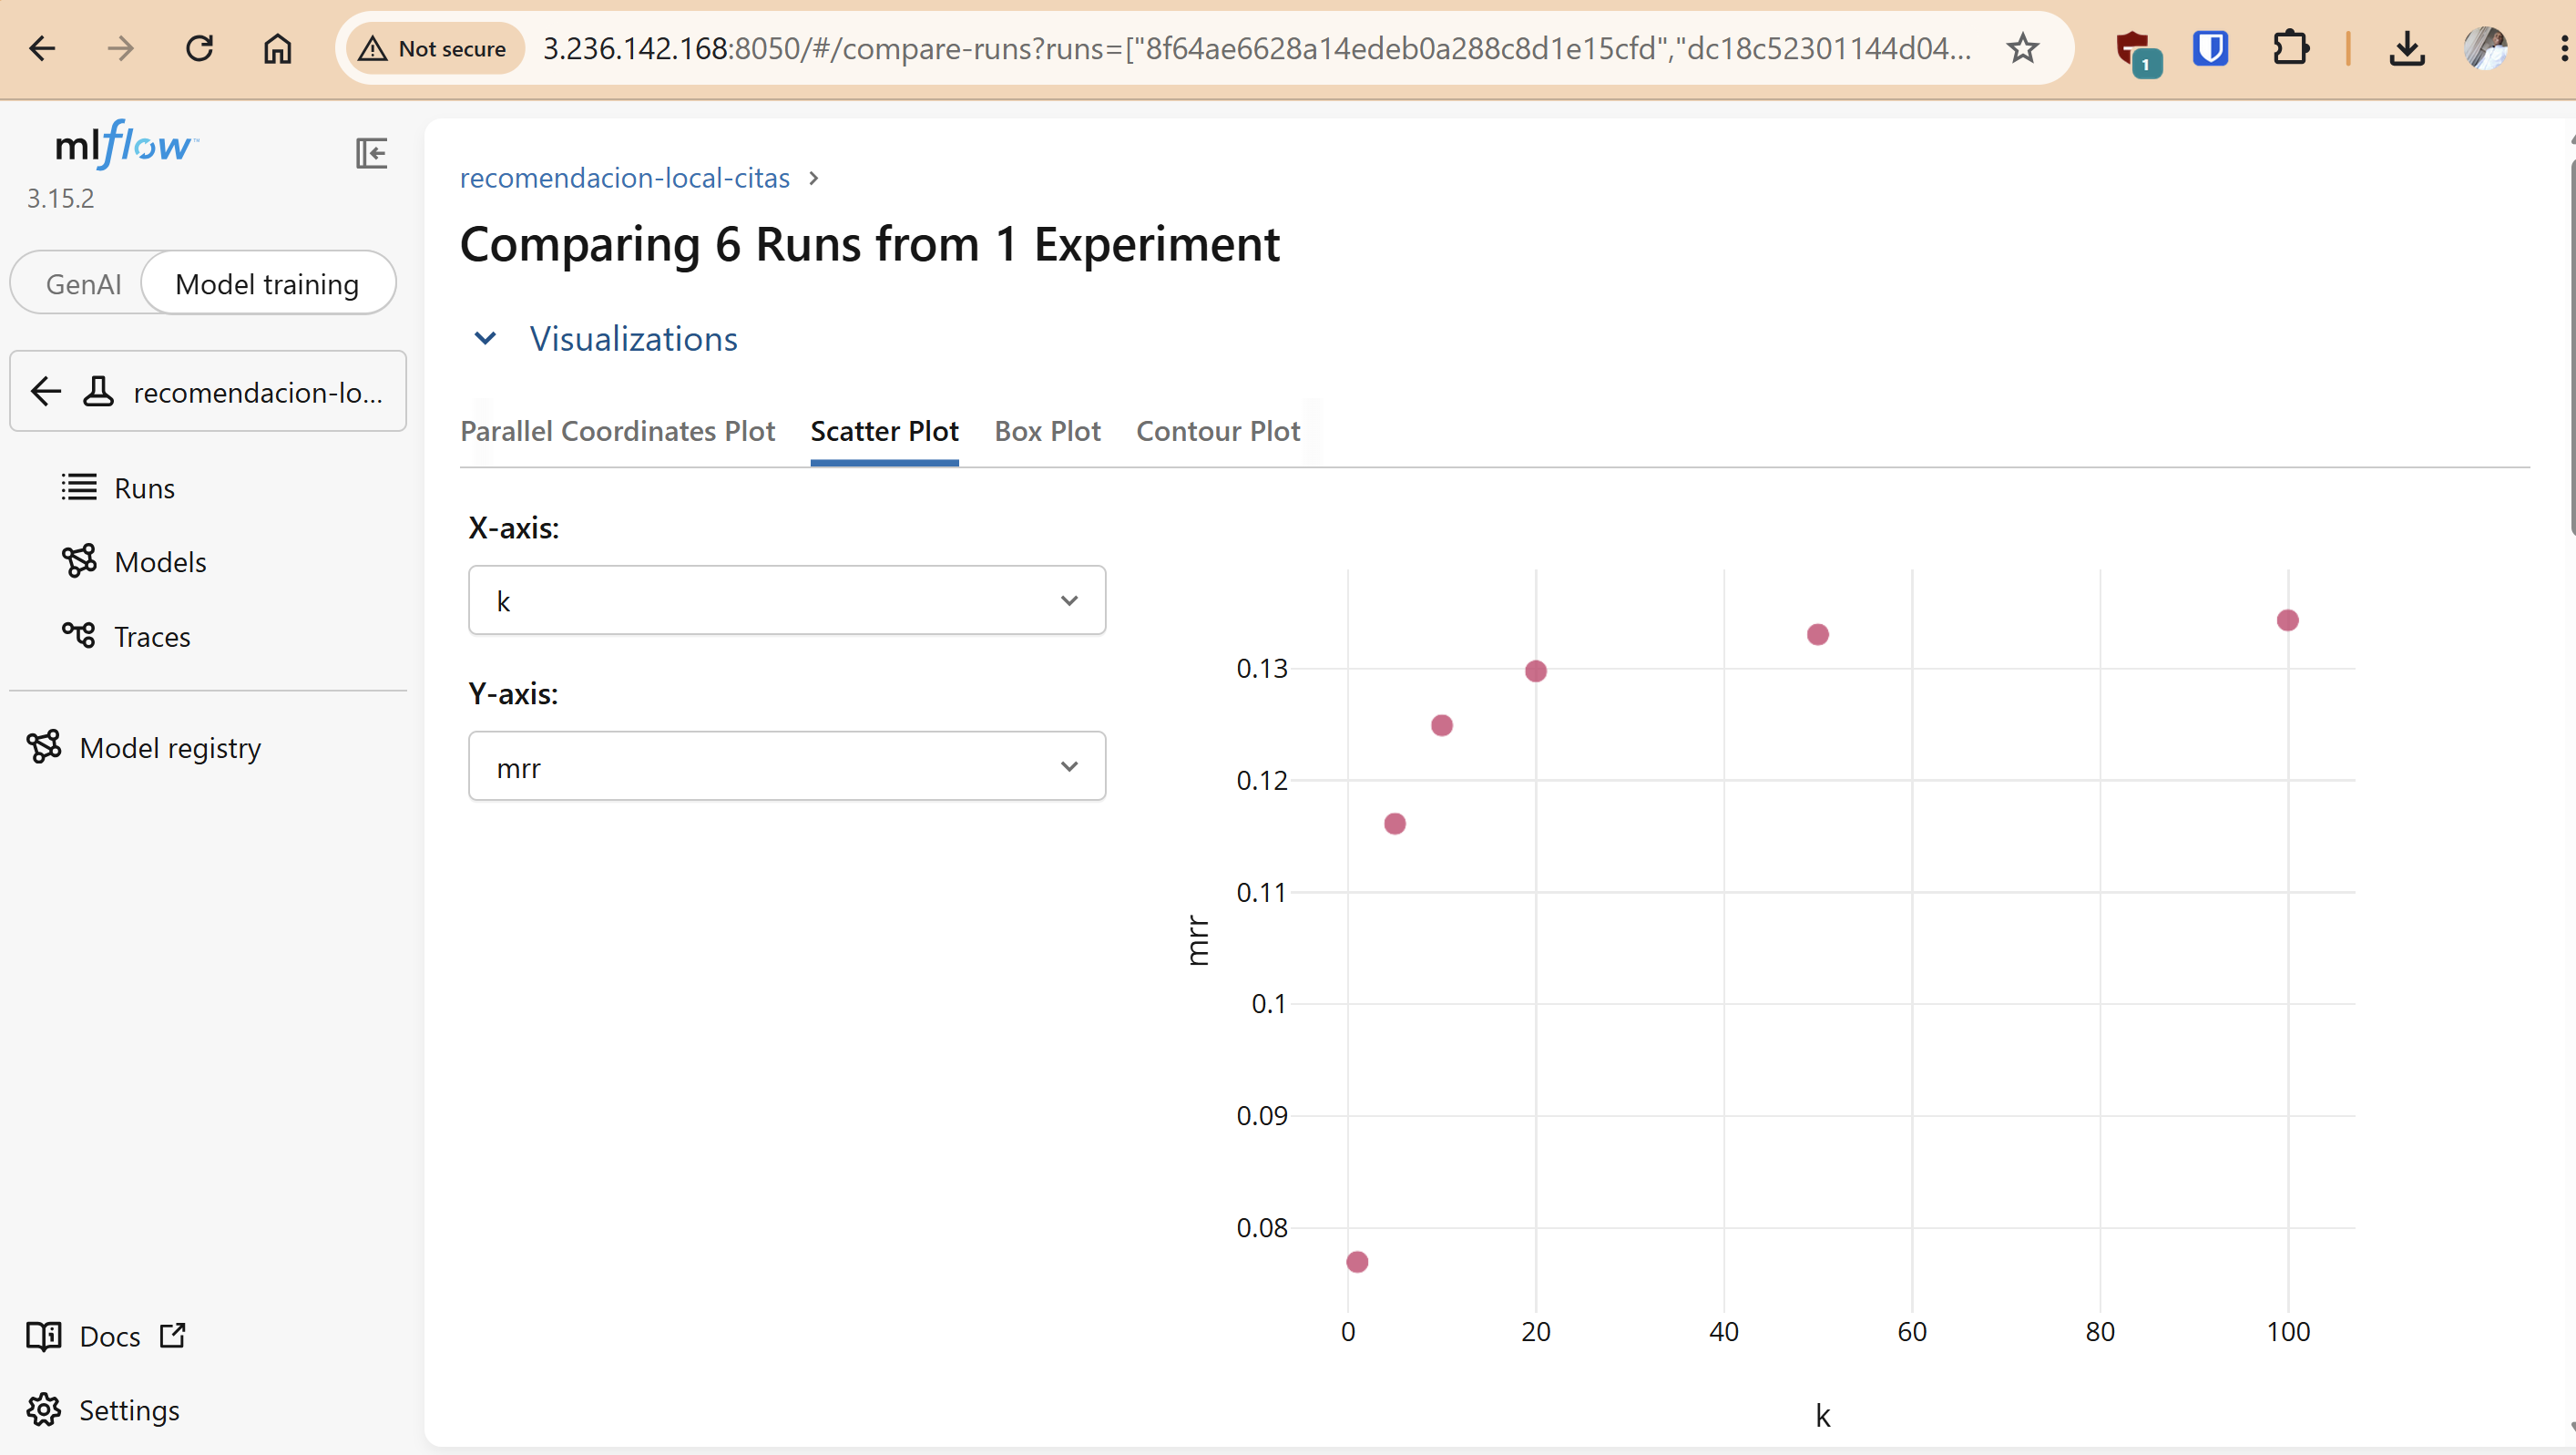
\includegraphics[width=0.48\textwidth]{mlflow_curva_mrr_k.png}
\caption{Recall@K (izquierda) y MRR@K (derecha) de la línea base en función de la profundidad del ranking. El Recall crece de forma sostenida mientras el MRR se estabiliza a partir de $K=10$.}
\label{fig:curvas}
\end{figure}

\subsection{Efecto del tamaño del vocabulario}

Se evaluaron dos variantes con $K=10$, modificando una sola condición cada vez:

\begin{table}[h!]
\centering
\small
\caption{Sensibilidad de la línea base al tamaño del vocabulario}
\label{tab:vocab}
\begin{tabular}{l c c c c}
\toprule
\textbf{Variante} & \textbf{max\_features} & \textbf{min\_df} & \textbf{Vocabulario} & \textbf{Recall@10} \\
\midrule
Referencia          & 50.000 & 2 & 25.305 & 0,2541 \\
Vocabulario acotado & 10.000 & 2 & 10.000 & 0,2350 \\
Filtro más estricto & 50.000 & 5 & 13.834 & 0,2417 \\
\bottomrule
\end{tabular}
\end{table}

Reducir el vocabulario en un 60\,\% cuesta apenas un 7,5\,\% de Recall, lo que indica rendimientos decrecientes y ofrece margen para acotar el consumo de memoria en el despliegue.

\subsection{Reordenador supervisado con regresión logística}

Se implementó un modelo de segunda etapa que asigna una probabilidad de relevancia a cada par contexto--artículo y reordena los 100 candidatos recuperados por TF--IDF. Sus cinco variables son la similitud TF--IDF del contexto con el título y con el resumen, y las longitudes del contexto, título y resumen. Un \texttt{Pipeline} de scikit--learn estandariza estas variables y ajusta una regresión logística. La evaluación conserva los candidatos originales: por ello Recall@100 debe permanecer constante y sirve también como control de integridad.

Se compararon dos conjuntos de entrenamiento con 30.390 consultas, un positivo y dos negativos por consulta. La variante \emph{aleatoria} muestrea los negativos del catálogo completo; la variante \emph{difícil} toma los dos primeros resultados incorrectos del Top--100 TF--IDF. Ambos modelos se evaluaron sobre las mismas 9.381 consultas de validación, con la misma semilla y los mismos candidatos. Para esta comparación se recalculó TF--IDF sobre el Top--100 y se excluyó el artículo citante; este protocolo explica la pequeña diferencia frente a los valores generales de la Tabla~\ref{tab:curva}.

\begin{table}[h!]
\centering
\small
\caption{Comparación del reordenamiento sobre el mismo Top--100 de validación}
\label{tab:supervisado}
\begin{tabular}{l c c c}
\toprule
\textbf{Método} & \textbf{Recall@10} & \textbf{MRR@10} & \textbf{Recall@100} \\
\midrule
TF--IDF sin reordenar             & 0,2571 & 0,1339 & 0,5160 \\
Regresión logística, aleatorios   & \textbf{0,2882} & \textbf{0,1490} & 0,5160 \\
Regresión logística, difíciles    & 0,0629 & 0,0212 & 0,5160 \\
\bottomrule
\end{tabular}
\end{table}

La variante aleatoria mejora 0,0311 puntos de Recall@10 (12,1\,\% relativo) y 0,0151 de MRR@10 (11,3\,\% relativo) frente a su línea base comparable. En cambio, usar exclusivamente los negativos más difíciles invierte una señal central: su similitud media con el resumen es 0,2726, frente a 0,1295 en los positivos. La regresión asigna entonces un coeficiente negativo a esa similitud ($-2{,}09$) y degrada el orden. El experimento muestra que \emph{más difícil} no significa automáticamente \emph{mejor}: con solo cinco variables, los negativos difíciles son léxicamente más parecidos que el artículo citado y el modelo no dispone de señales semánticas suficientes para distinguirlos.

Como Recall@100 es 0,5160 en las tres filas, la caída no se debe a pérdida de candidatos sino únicamente al orden aprendido. Para esta entrega se selecciona la variante con negativos aleatorios. Como extensión se propone mezclar negativos aleatorios y difíciles, o incorporar representaciones semánticas, en lugar de usar exclusivamente los dos falsos positivos más altos.

\subsection{Registro de experimentos en MLflow}

El equipo dispone de un servidor MLflow desplegado sobre una instancia EC2 (Ubuntu 26.04, \texttt{t3.small}), accesible en el puerto 8050. La configuración está centralizada en \path{src/tracking/mlflow_setup.py}, de modo que todos los experimentos comparten el mismo nombre y las mismas claves de métricas, condición necesaria para que las comparaciones sean válidas. Las corridas supervisadas se repitieron con \path{MLFLOW_TRACKING_URI} apuntando a ese servidor, junto con una verificación de sensibilidad a la regularización (\texttt{c} = 0,1 / 1,0 / 10,0 para cada estrategia de negativos): el valor de \texttt{c} no cambia la conclusión en ningún caso, lo que confirma que el colapso de la variante difícil no se debe a la regularización sino a la señal invertida descrita más abajo.

\begin{figure}[h!]
\centering
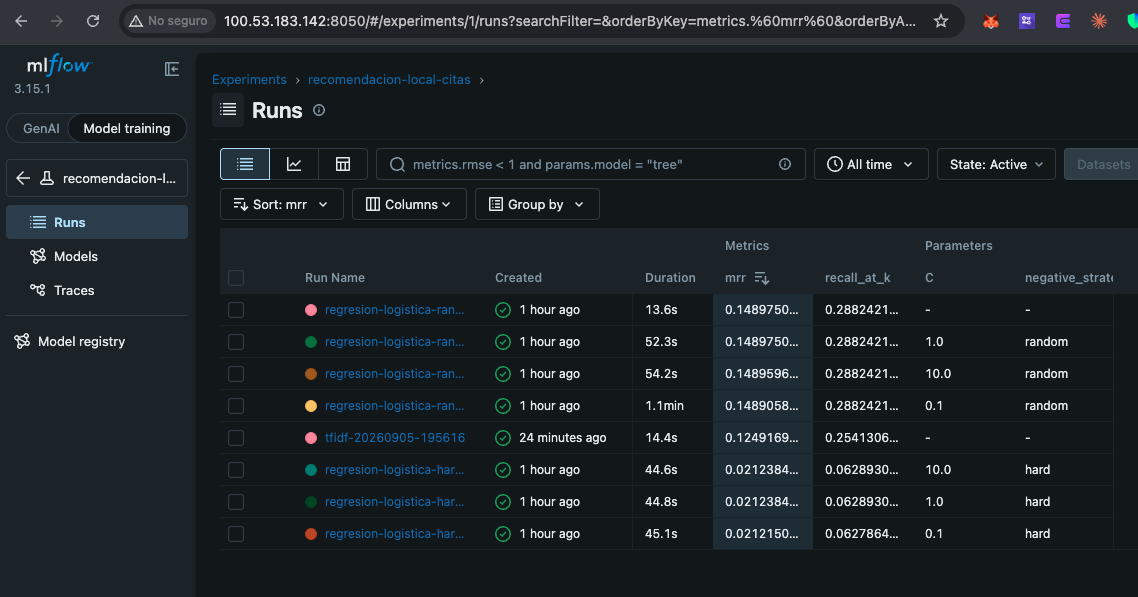
\includegraphics[width=0.92\textwidth]{mlflow_tabla_runs.png}
\caption{Corridas registradas en el servidor MLflow compartido: línea base y las seis combinaciones supervisadas (dos estrategias de negativos por tres valores de \texttt{c}), con Recall@10 y MRR@10 visibles para cada una.}
\label{fig:runs}
\end{figure}

\begin{figure}[h!]
\centering
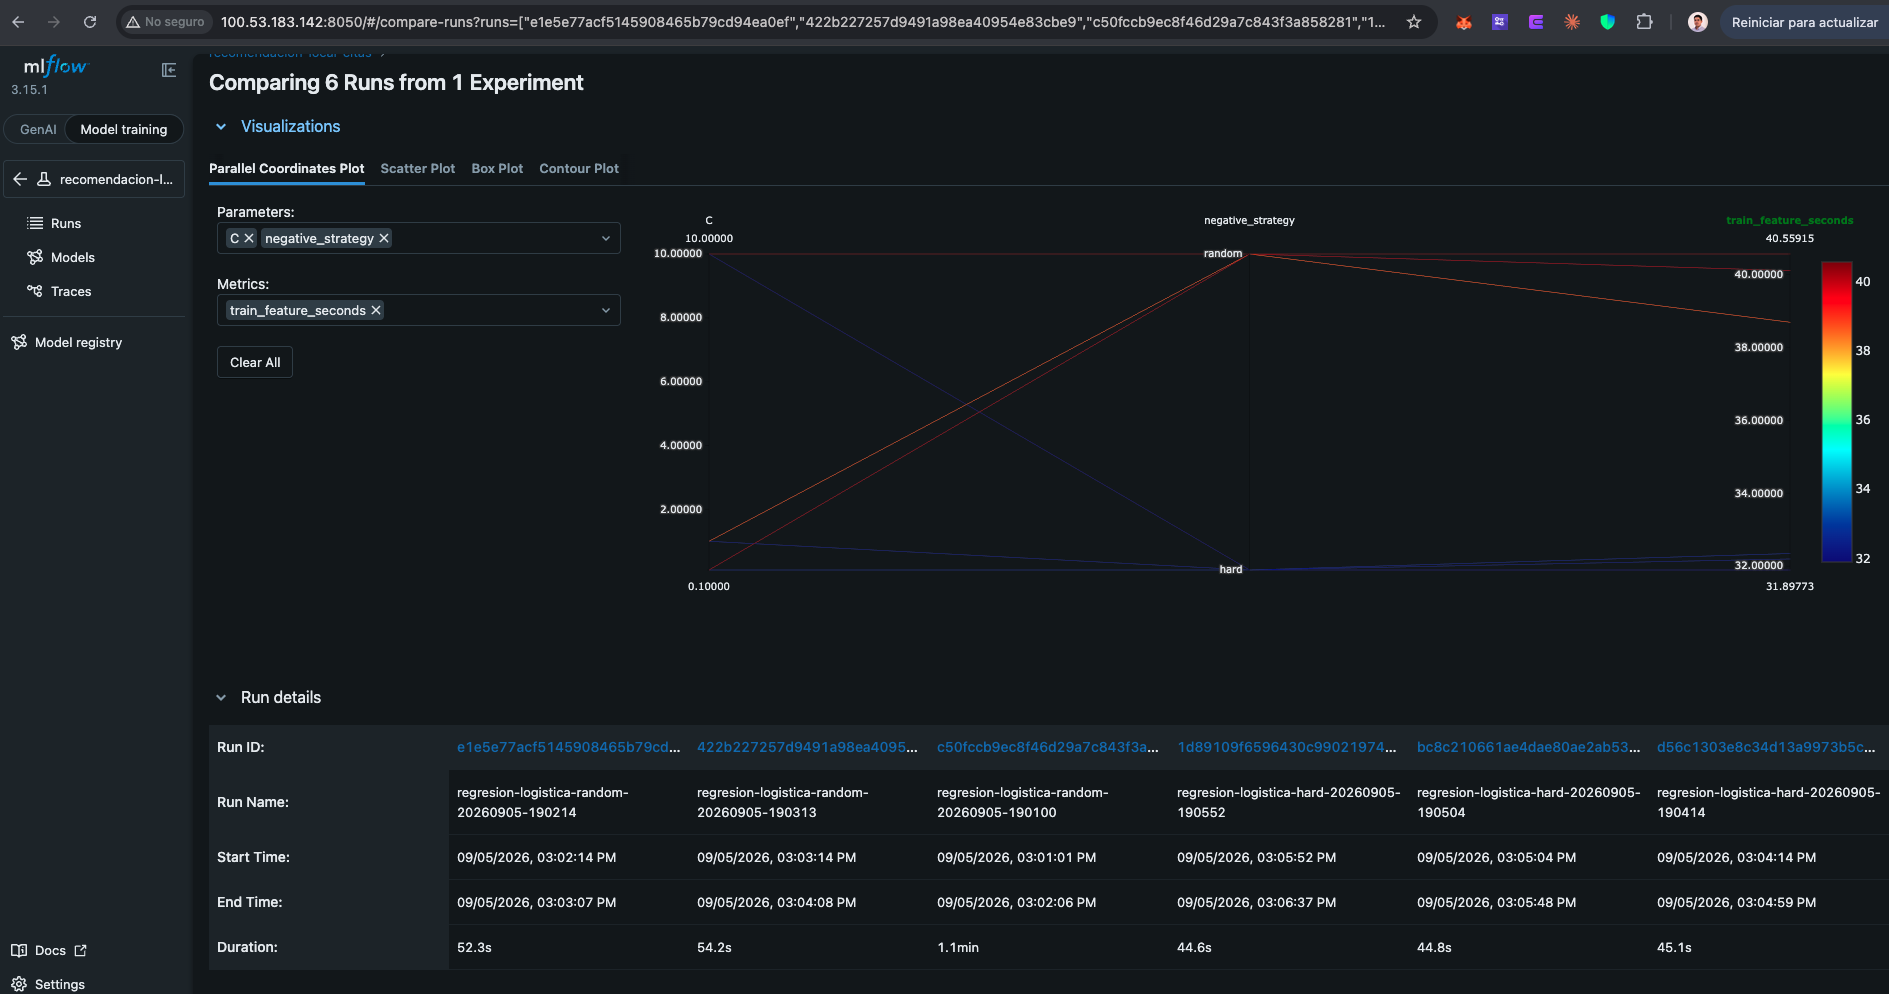
\includegraphics[width=0.85\textwidth]{mlflow_boxplot_estrategia.png}
\caption{Comparación generada en MLflow (\emph{Compare Runs} $\rightarrow$ \emph{Box Plot}) de MRR@10 agrupado por estrategia de negativos sobre las seis corridas supervisadas. Los tres valores de \texttt{c} quedan agrupados dentro de cada categoría, evidenciando que la brecha depende de la estrategia y no de la regularización.}
\label{fig:boxplot}
\end{figure}

% ============================================================================
% 3. OBSERVACIONES Y CONCLUSIONES
% ============================================================================
\section{Observaciones y conclusiones sobre los modelos}

\subsection{El techo del sistema de dos etapas}

Recall@100 $=0{,}5163$ es el resultado más consecuente de esta entrega. Como la segunda etapa solo reordena los candidatos que la primera recupera, \textbf{ningún reordenador puede superar ese 51,6\,\%} mientras la recuperación siga siendo puramente léxica. Elevar ese techo exige actuar sobre la primera etapa, no sobre la segunda: representaciones semánticas basadas en \textit{embeddings} de textos científicos son la vía natural, y quedan planteadas para la Entrega 3.

\subsection{Los aciertos existen pero están mal ubicados}

El contraste entre las dos curvas de la Figura~\ref{fig:curvas} es revelador. Al pasar de $K=10$ a $K=100$ el Recall se duplica (0,2541 a 0,5163) mientras el MRR apenas se mueve (0,1249 a 0,1343, un 7,5\,\%). Esto significa que los artículos recuperados entre las posiciones 10 y 100 quedan tan abajo que casi no aportan al ranking.

Es exactamente el escenario donde un reordenamiento supervisado aporta valor: no necesita encontrar nada nuevo, solo subir lo que la primera etapa ya recuperó. La brecha entre Recall@100 y MRR@100 cuantifica ese margen disponible.

\subsection{Implicaciones para el diseño}

\begin{itemize}[leftmargin=1.4em, itemsep=1pt, topsep=2pt]
  \item \textbf{Profundidad de recuperación.} La ganancia de Recall se desacelera después de $K=50$. Recuperar 100 candidatos parece un punto razonable entre cobertura y costo de reordenamiento.
  \item \textbf{Costo de la primera etapa.} La evaluación completa sobre 9.381 consultas toma unos 13 segundos en lote, pero una API debe responder una consulta en tiempo interactivo. La arquitectura en dos etapas es lo que hace viable ese requisito.
  \item \textbf{Vocabulario.} Puede acotarse de forma significativa con una pérdida menor de desempeño, lo que reduce la memoria del artefacto desplegado.
\end{itemize}

La comparación de la Tabla~\ref{tab:supervisado} confirma que el reordenamiento puede aprovechar parte de ese margen: la variante aleatoria supera a TF--IDF en Recall@10 y MRR@10. Por tanto, es el modelo seleccionado para empaquetar en la Entrega 3. La variante de negativos difíciles se conserva como resultado experimental y como diagnóstico de una limitación: la similitud léxica por sí sola no permite separar adecuadamente artículos temáticamente cercanos.

% ============================================================================
% 4. TABLERO DESARROLLADO
% ============================================================================
\section{Descripción del tablero desarrollado}

El prototipo de la Entrega 2 se implementó en \texttt{src/app/} como una aplicación web integrada. El backend utiliza FastAPI y el frontend se sirve desde el mismo proceso, permitiendo ejecutar localmente la solución mediante el comando \texttt{uv run tablero}. Durante el arranque se carga la línea base TF--IDF sobre los 19.776 artículos del corpus y se precalcula o recupera la información utilizada en las visualizaciones.

\subsection{Recomendador de citas}

El panel principal recibe un fragmento académico en inglés y permite seleccionar la cantidad de resultados que se desea recuperar. Al presionar \emph{Recomendar citas}, el frontend envía la consulta al endpoint \texttt{POST /api/recomendar}. El backend transforma el contexto con el mismo vectorizador TF--IDF empleado durante la evaluación, calcula la similitud coseno contra el corpus y devuelve el ranking de artículos.

Cada recomendación presenta posición, título, identificador y puntaje de similitud. Al seleccionar un artículo, el tablero muestra además un extracto de su resumen. El botón \emph{Usar un ejemplo real} obtiene un contexto auténtico del corpus mediante \texttt{GET /api/ejemplo}, lo que permite probar la aplicación con una consulta reproducible.

\notabox{\textbf{Alcance de la integración actual.} El tablero de esta entrega sirve la línea base TF--IDF, que ya produce recomendaciones reales. El reordenador supervisado con regresión logística fue desarrollado y evaluado en esta entrega, pero su integración como modelo de inferencia definitivo se deja para la Entrega 3, junto con su empaquetamiento.}

\subsection{Exploración y diagnóstico}

La zona inferior del tablero consolida resultados que antes se encontraban separados entre el cuaderno de exploración, las ejecuciones de evaluación y el reporte. Se organiza en tres pestañas:

\begin{itemize}[leftmargin=1.4em, itemsep=1pt, topsep=2pt]
  \item \textbf{Estudio de los datos}: presenta los 63.768 contextos, los 19.776 artículos candidatos, las particiones de entrenamiento, validación y prueba, distribuciones de longitud y comprobaciones de calidad.
  \item \textbf{Desempeño del modelo}: presenta Recall@K y MRR@K para diferentes profundidades del ranking. En validación se observan Recall@10 de 0,2541, MRR@10 de 0,1249 y Recall@100 de 0,5163.
  \item \textbf{Diagnóstico de negativos}: compara positivos, negativos aleatorios y negativos difíciles. El análisis evidencia que los negativos aleatorios son demasiado fáciles de separar mediante similitud léxica, mientras que los negativos difíciles representan un escenario de ranking sustancialmente más exigente.
\end{itemize}

Los datos del tablero se exponen mediante \texttt{GET /api/insights}, mientras \texttt{GET /api/estado} permite comprobar que el recomendador está cargado y reporta su configuración. Durante la validación final se comprobó la comunicación completa entre interfaz y backend, obteniendo respuestas HTTP 200 tanto para la carga de información como para una recomendación real.

\begin{figure}[h!]
\centering
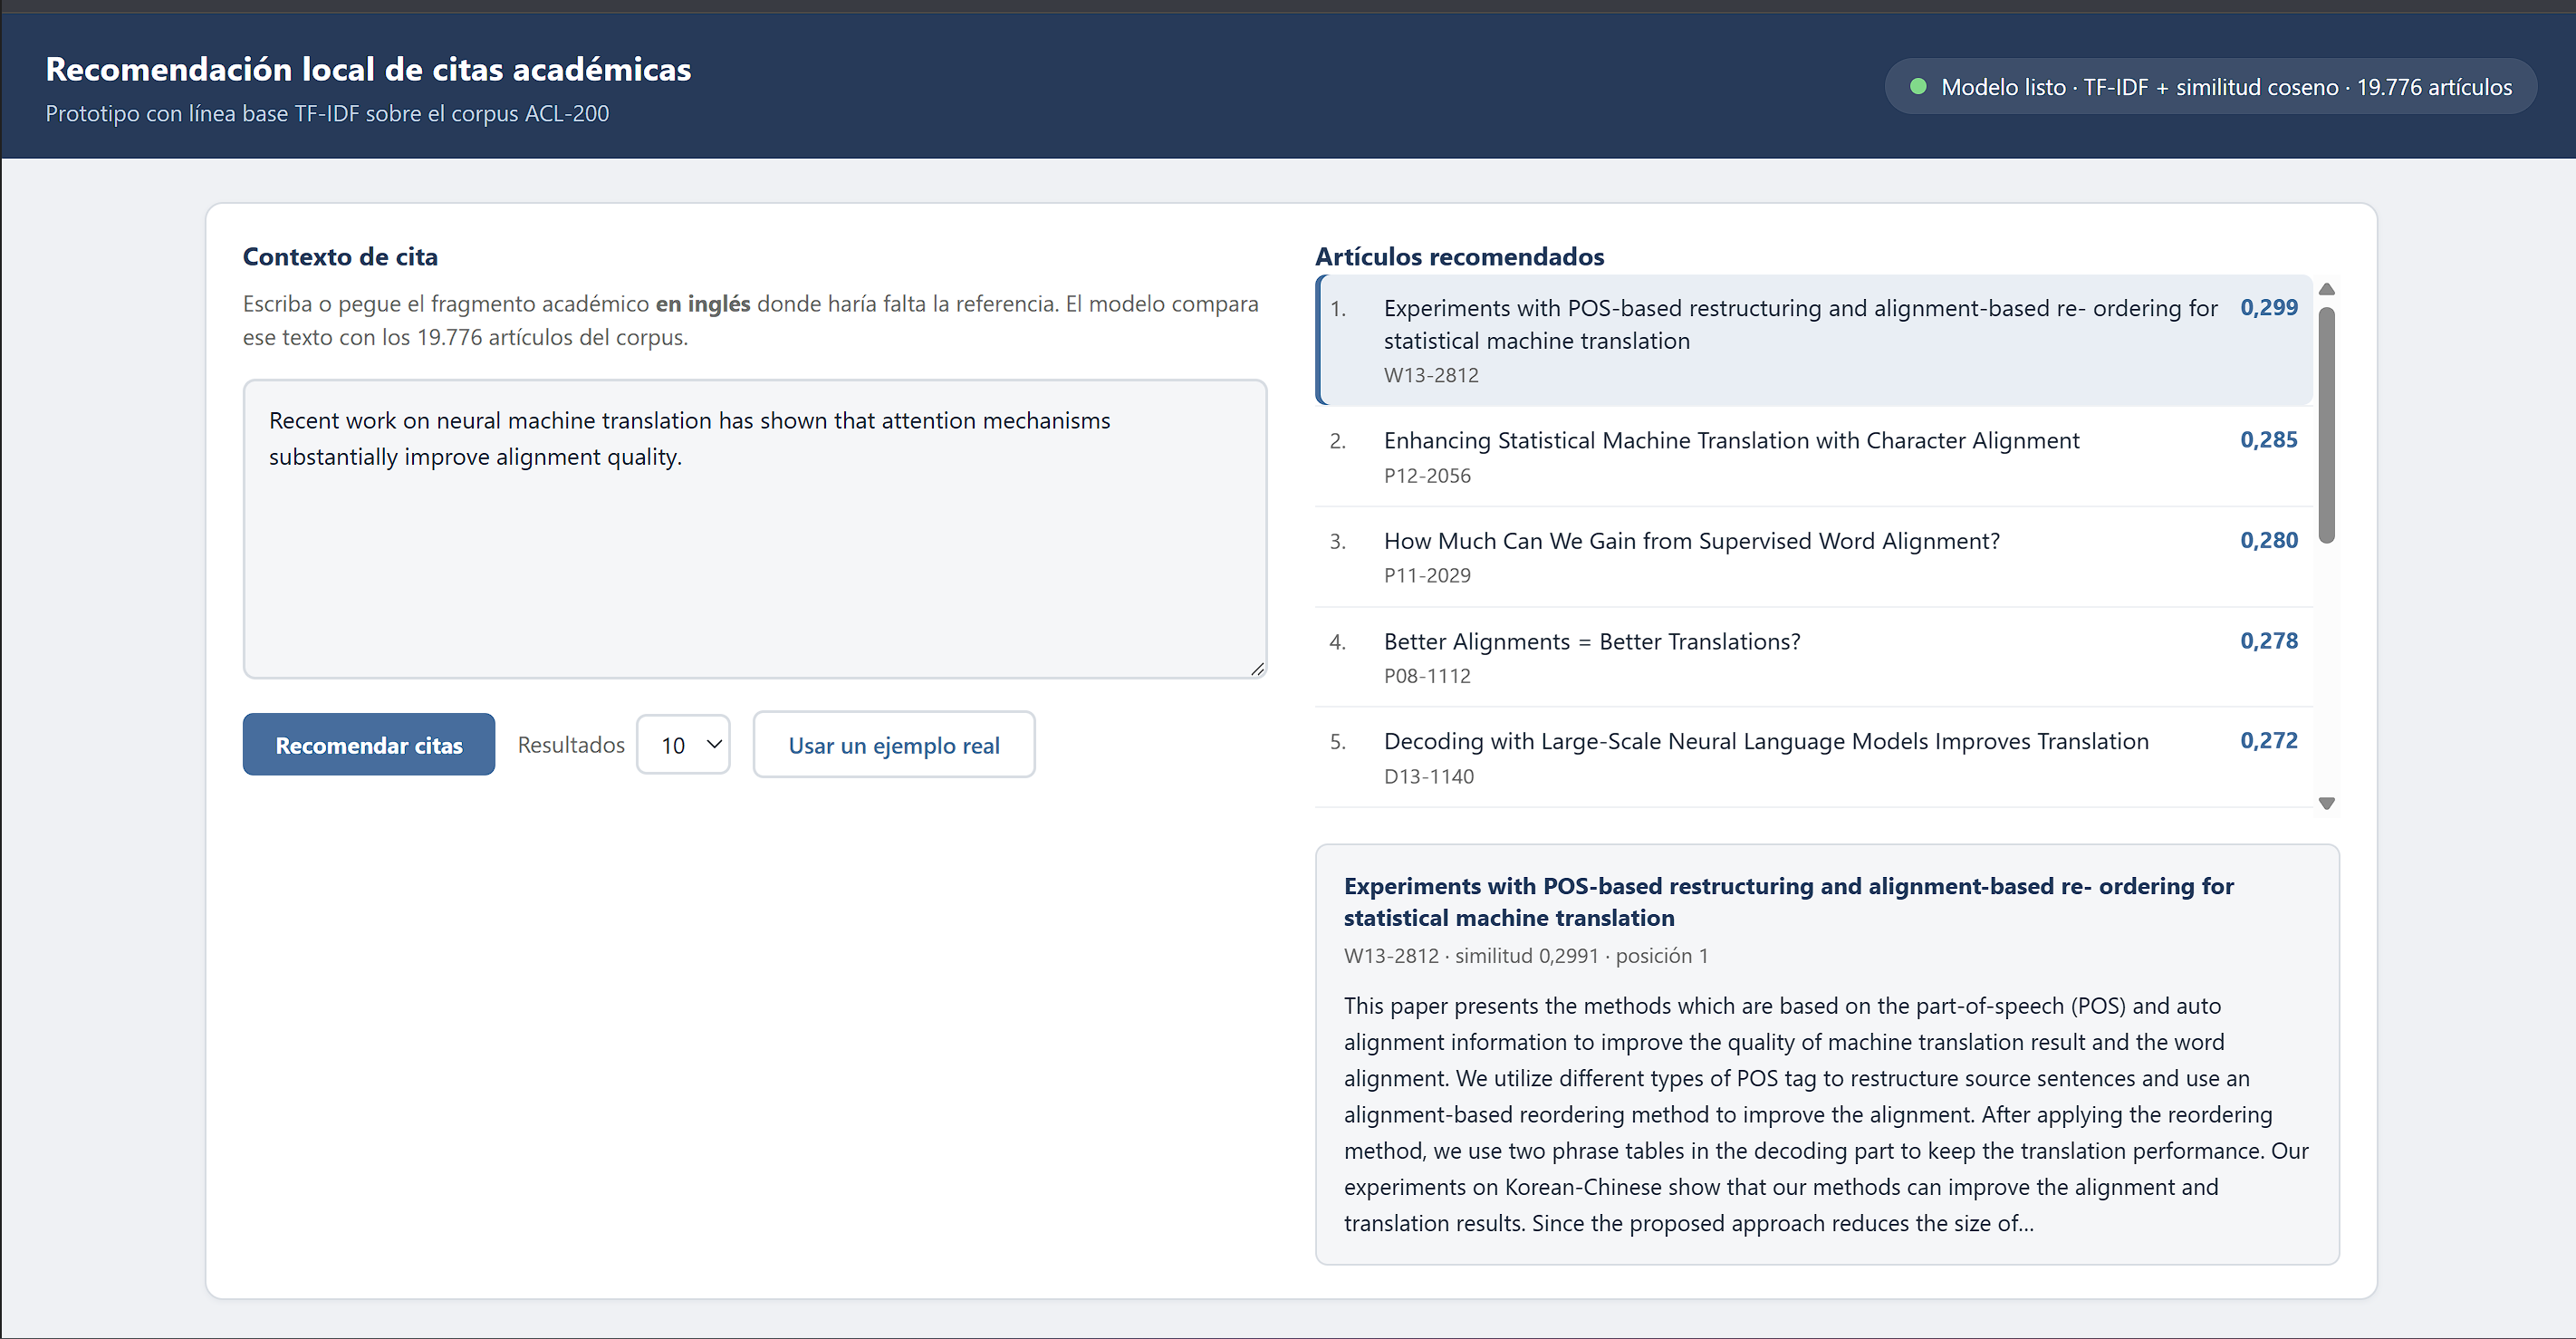
\includegraphics[width=0.95\textwidth]{tablero_recomendacion_real.png}
\caption{Tablero del prototipo ejecutando una consulta académica real y mostrando el ranking de artículos recomendados por la línea base TF--IDF.}
\label{fig:tablero}
\end{figure}

% ============================================================================
% EVIDENCIAS
% ============================================================================
\section{Evidencias y soportes}

\subsection{Repositorio de código}

\begin{center}
\url{https://github.com/Byron971/microproyecto-local-citation}
\end{center}

Las fuentes de los modelos se encuentran en \texttt{src/models/} y \texttt{src/training/}; la evaluación en \texttt{src/evaluation/}; el seguimiento experimental en \texttt{src/tracking/}; y el tablero funcional con su backend y frontend en \texttt{src/app/}. El historial de \textit{commits} y los \textit{Pull Requests} evidencian la contribución de cada integrante.

\subsection{Infraestructura de experimentación en AWS}

Cada integrante trabajó desde su propia cuenta de AWS Academy; las siguientes capturas evidencian instancias EC2 reales ejecutando MLflow, con usuario e IP visibles en cada caso.

\begin{figure}[h!]
\centering
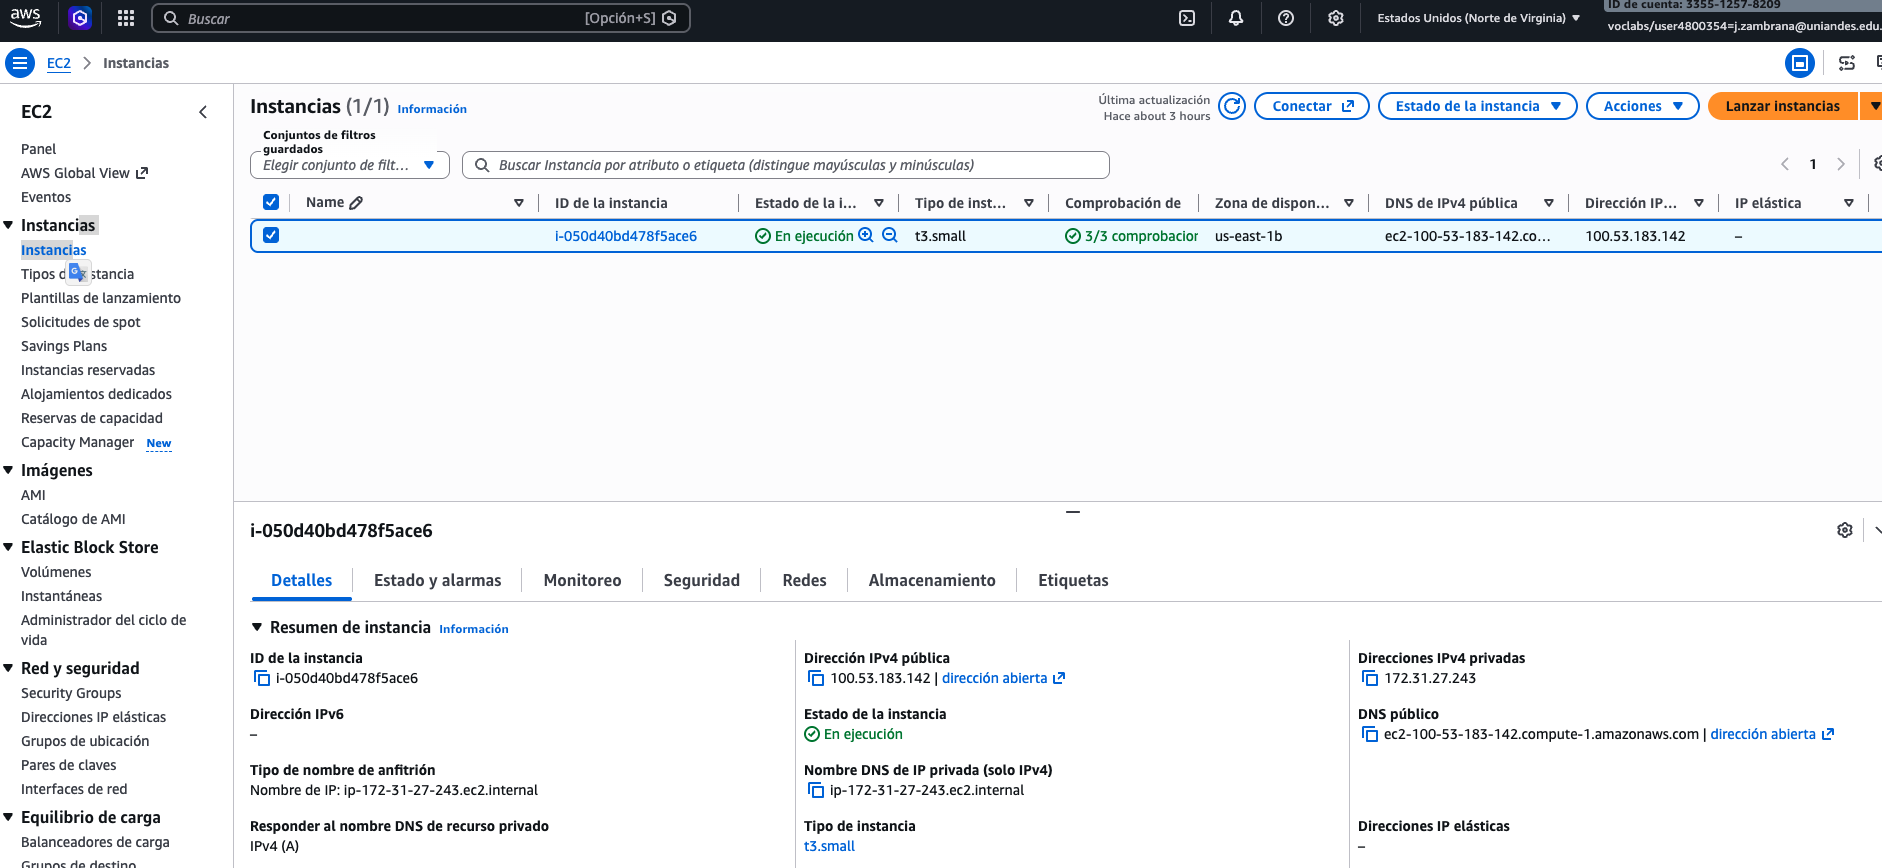
\includegraphics[width=0.48\textwidth]{ec2_instancia.png}
\hfill
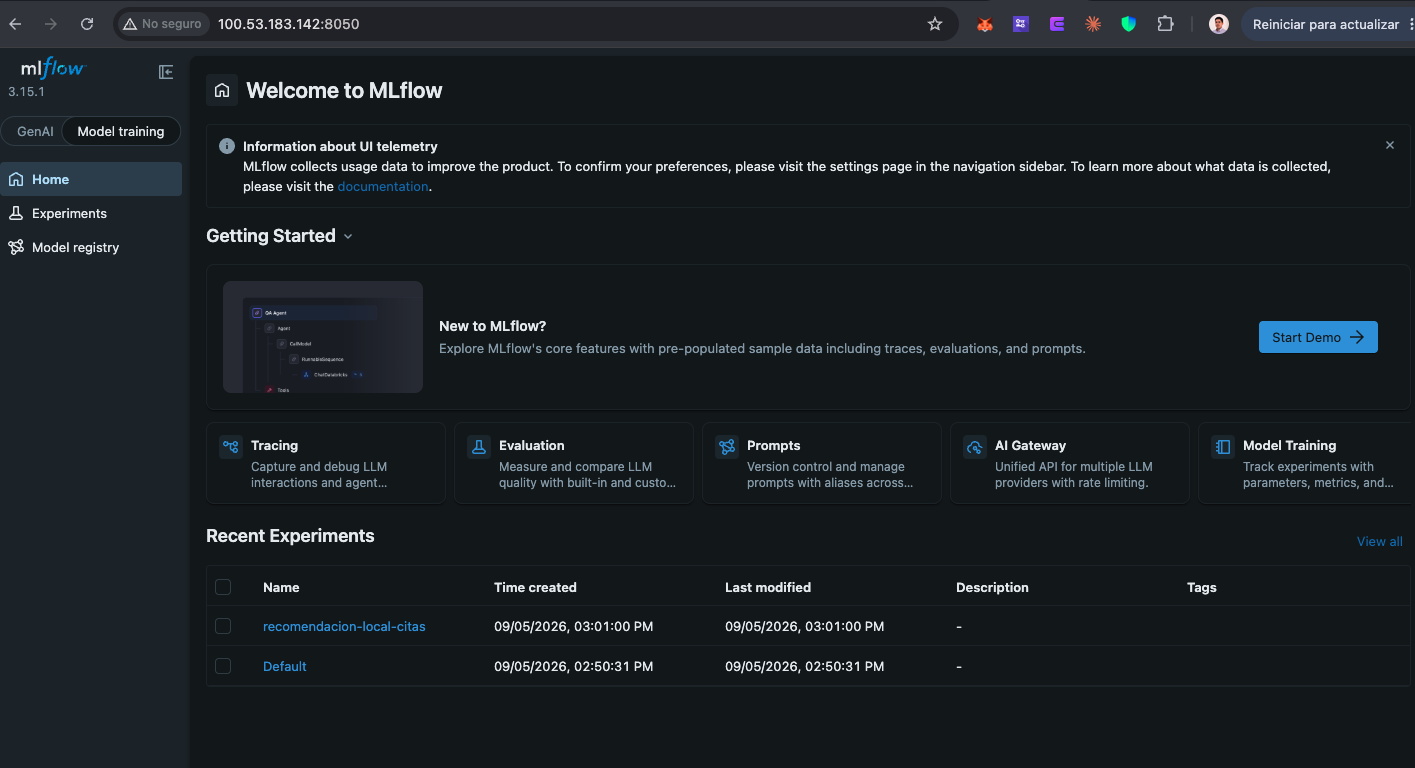
\includegraphics[width=0.48\textwidth]{mlflow_ui_ip.png}
\caption{Instancia EC2 de José Zambrana en ejecución --usuario de AWS Academy, IP pública y privada visibles-- (izquierda) y esa misma IP sirviendo la interfaz de MLflow en el navegador (derecha).}
\label{fig:ec2}
\end{figure}

\begin{figure}[h!]
\centering
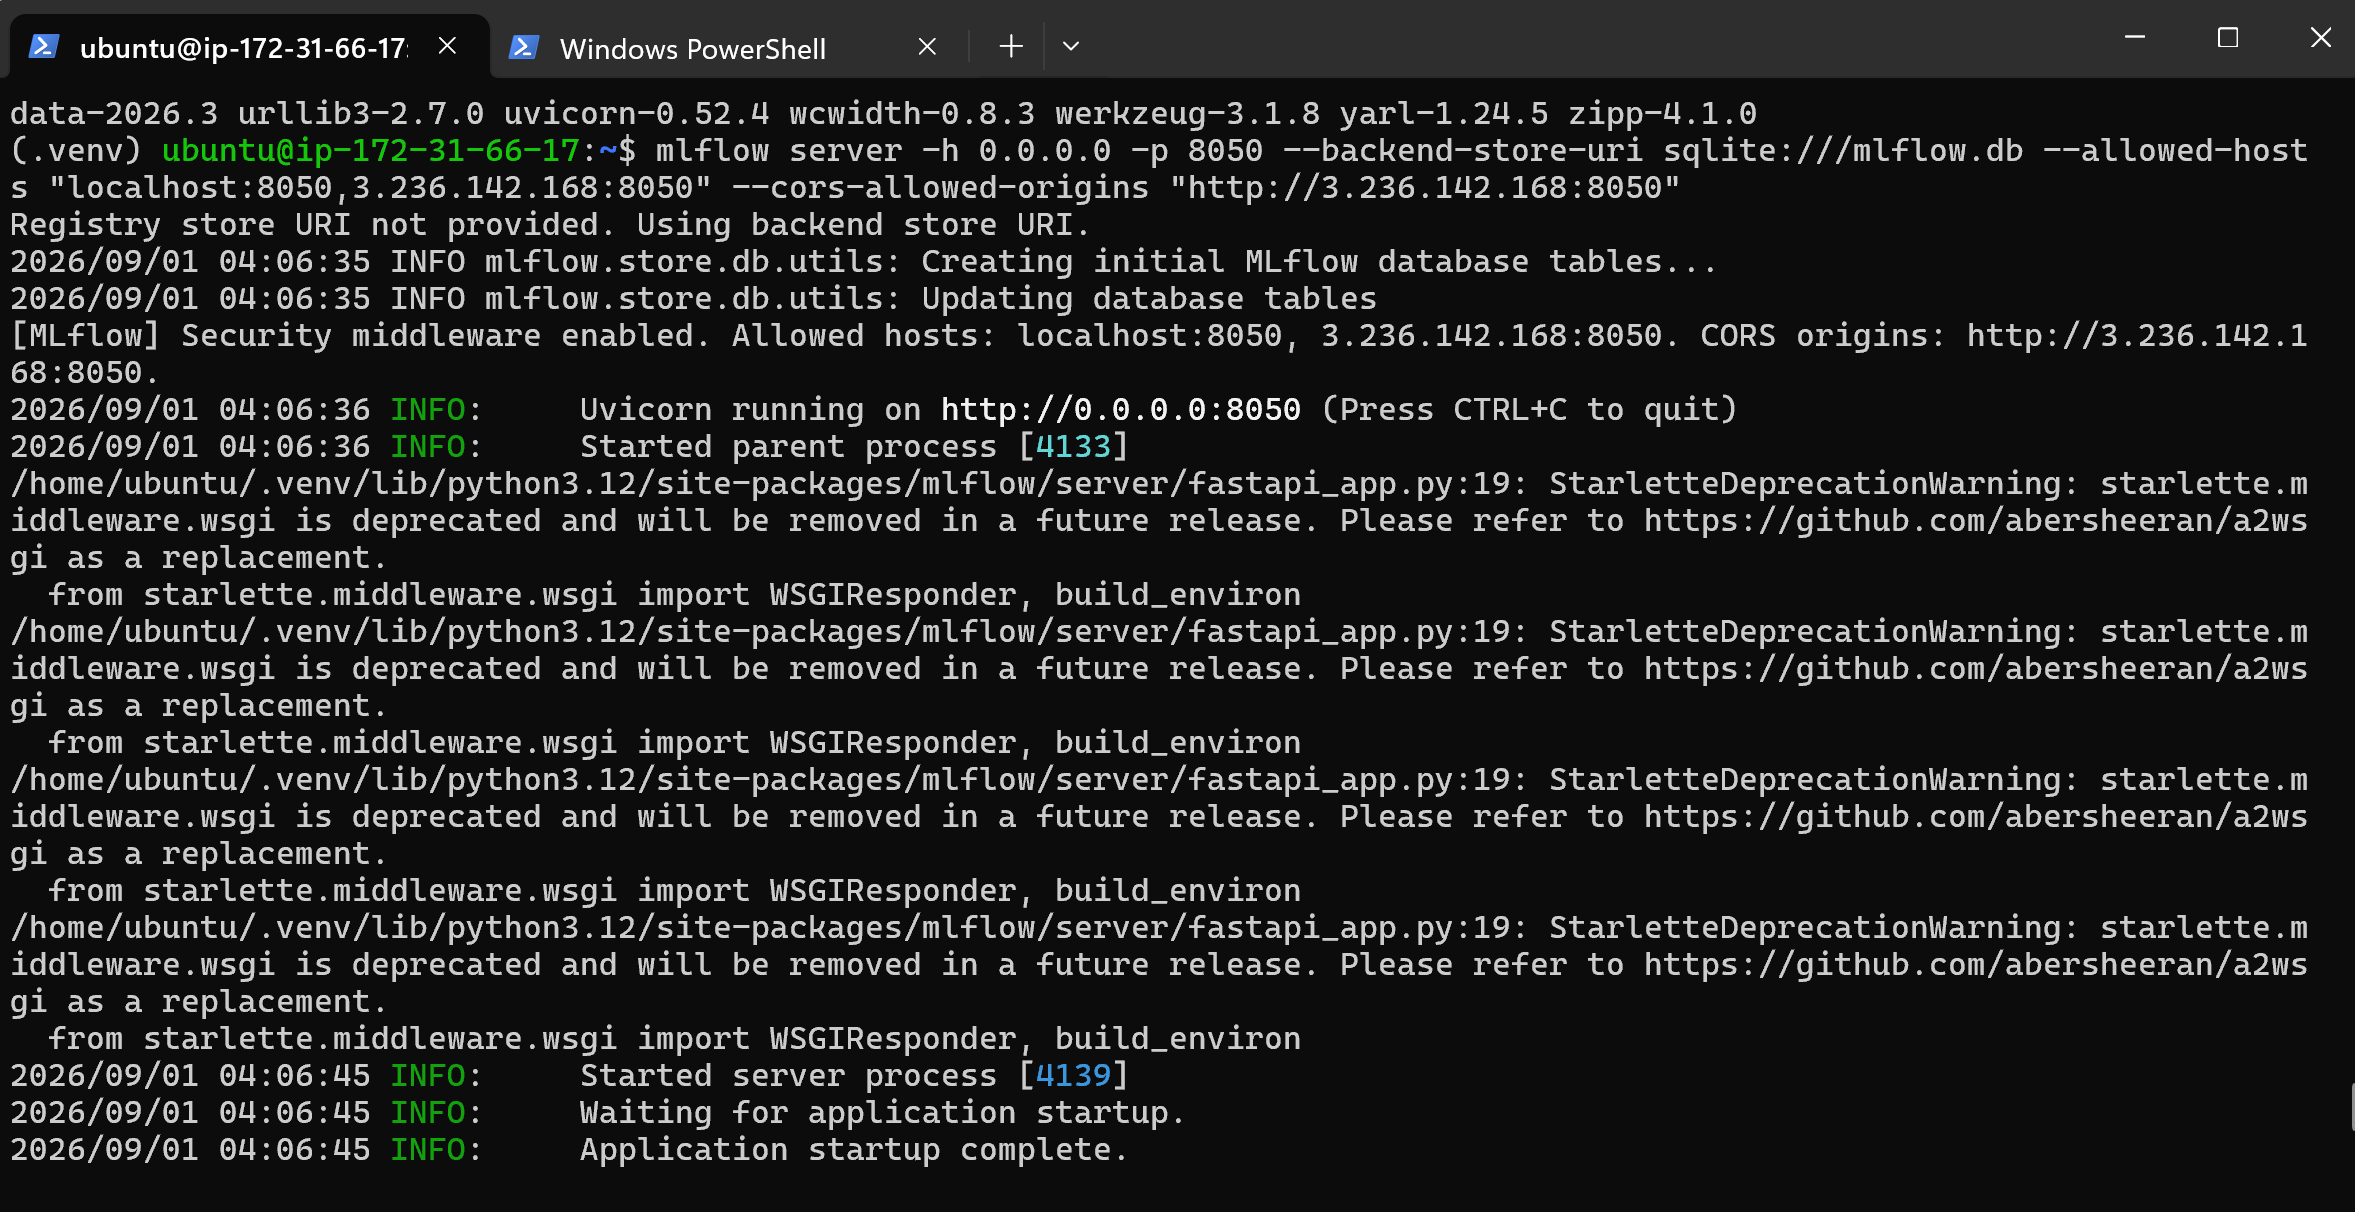
\includegraphics[width=0.65\textwidth]{ec2_mlflow_servidor.png}
\caption{Servidor de MLflow desplegado originalmente por Carlos Caicedo sobre su propia instancia EC2, expuesto en el puerto 8050.}
\label{fig:servidor}
\end{figure}

% ============================================================================
% REPORTE DE TRABAJO EN EQUIPO
% ============================================================================
\clearpage
\section{Reporte de trabajo en equipo}

El equipo distribuyó las actividades de esta entrega en cuatro frentes: el pipeline de datos supervisados, la infraestructura de seguimiento de experimentos, el desarrollo y la evaluación de los modelos, y el tablero. La coordinación se realizó de forma asíncrona mediante \textit{issues} agrupados en hitos con fecha límite, y la integración a la rama principal se hizo a través de \textit{Pull Requests} revisados por los demás integrantes, con un archivo \texttt{CODEOWNERS} que solicita automáticamente la revisión de todo el equipo. La Tabla~\ref{tab:equipo} resume el aporte de cada integrante, respaldado por sus propios \textit{commits} en el historial de Git.

\begin{table}[h!]
\centering
\caption{Aportes verificables en el repositorio}
\label{tab:equipo}
\small
\begin{tabular}{p{2.9cm} p{11.4cm}}
\toprule
\textbf{Integrante} & \textbf{Aporte y evidencia registrada} \\
\midrule

John Arias &
Pipeline de datos supervisados: carga de los conjuntos, generación reproducible de pares positivos y negativos con semilla fija, versionamiento de los conjuntos procesados con DVC y métricas de evaluación de ranking (Recall@K y MRR). Integración de contribuciones y validación reproducible del flujo del proyecto. \\[3pt]

Carlos Caicedo &
Infraestructura de seguimiento de experimentos con MLflow, incluido su despliegue sobre una instancia AWS EC2 y la configuración centralizada de convenciones de experimentos y métricas. Línea base TF--IDF con similitud coseno, su evaluación sobre las 9.381 consultas de validación y el barrido de corridas registradas en el servidor. Restauración y documentación de remotos de DVC. \\[3pt]

José Zambrana &
Modelo supervisado de relevancia (\textit{issue} \#6): extracción de características contexto--artículo, generación reproducible de negativos difíciles, reordenador con regresión logística, comparación de estrategias mediante Recall@K y MRR, registro de modelos y resultados en MLflow, y pruebas automatizadas con pytest y Tox. En la Entrega 1 aportó la exploración de datos y su cuaderno. \\[3pt]

Carlos Duque &
Desarrollo del tablero funcional conforme a la maqueta aprobada y conexión con datos reales del EDA (\textit{issues} \#8 y \#9). Implementó el backend y frontend integrados en \texttt{src/app/}, la visualización de métricas y diagnósticos, y el flujo de recomendación basado en el modelo TF--IDF. Su contribución fue integrada a \texttt{main} mediante el Pull Request \#28 durante la ventana de esta entrega. \\
\bottomrule
\end{tabular}
\end{table}

\vspace{-4pt}
\noindent\footnotesize\textit{Ventana considerada: del 24 de agosto al 6 de septiembre de 2026, correspondiente al periodo de trabajo de la Entrega 2. La verificación se realizó sobre el historial de ramas, commits y Pull Requests del repositorio, considerando las contribuciones integradas durante el periodo.}\normalsize

\vspace{6pt}

El reparto de tareas quedó registrado en los \textit{issues} del repositorio, cada uno con su criterio de aceptación y la evidencia que lo respalda, de modo que el avance de cada integrante puede verificarse directamente sobre el repositorio. Los experimentos quedaron centralizados en un único servidor de MLflow, lo que permite comparar corridas de distintos integrantes bajo el mismo experimento y con las mismas métricas.

% ============================================================================
\section*{Referencias}
\addcontentsline{toc}{section}{Referencias}

\begin{list}{}{%
  \setlength{\leftmargin}{1.2cm}
  \setlength{\itemindent}{-1.2cm}
  \setlength{\itemsep}{8pt}
  \setlength{\parsep}{0pt}
}

\item Gu, N. (2022). \textit{Local-Citation-Recommendation} [Computer software]. GitHub. \url{https://github.com/nianlonggu/Local-Citation-Recommendation}

\item Gu, N., Gao, Y., \& Hahnloser, R.\,H.\,R. (2022). Local citation recommendation with hierarchical-attention text encoder and SciBERT-based reranking. In M. Hagen et al. (Eds.), \textit{Advances in Information Retrieval} (pp. 274--288). Springer International Publishing. \url{https://doi.org/10.1007/978-3-030-99736-6_19}

\item Treveil, M., \& Dataiku Team. (2021). \textit{Introducing MLOps: How to scale machine learning in the enterprise}. O'Reilly Media.

\end{list}

\end{document}
